\documentclass[xcolor={dvipsnames}]{beamer}

\usetheme{Malmoe}
\usecolortheme{seagull}
\usepackage[]{natbib}
\usepackage{textpos}
\usepackage{amsmath, amssymb, bm}
\usepackage{multirow}
\usepackage{framed}
\usepackage{schemata}
\setbeamertemplate{navigation symbols}{}
\usepackage[english]{babel}
\usepackage{graphics}
\usepackage{fontawesome}
\usepackage{xcolor}
\usepackage[export]{adjustbox}
\usepackage{tikz,graphicx,animate}

\definecolor{lightpink2}{rgb}{0.145,0.6666,1} % Defines the color used for content box headers
\definecolor{Red}{rgb}{0.9,0.15,0}
\definecolor{pink2}{RGB}{55,126,184}
\definecolor{Green}{RGB}{77,175,74}
\definecolor{White}{RGB}{255,255,255}
\definecolor{Lightgray}{rgb}{0.86,0.86,0.86}
\definecolor{pink2}{rgb}{1.0, 0.33, 0.64}
\definecolor{blue2}{rgb}{0.0, 0.53, 0.74}
%\definecolor{Mycolor1}{HTML}{CABED0}
%\definecolor{Mycolor9}{HTML}{3F2949}

\setbeamertemplate{footline}
{
	\leavevmode%
	\hbox{%
		\begin{beamercolorbox}[wd=.50\paperwidth,ht=2.25ex,dp=1ex,center]{author in head/foot}%
			\usebeamerfont{author in head/foot}\insertshortauthor%% \beamer@ifempty{\insertshortinstitute}{}{(\insertshortinstitute)}
		\end{beamercolorbox}%
%		\hskip2pt%
		\begin{beamercolorbox}[wd=.50\paperwidth,ht=2.25ex,dp=1ex,center]{title in head/foot}%
			\usebeamerfont{title in head/foot}\insertshorttitle~~~~~~~~~~~~~~~~~~~~~~~~~~\insertframenumber
		\end{beamercolorbox}%
	}%
	\vskip0pt%
}
\makeatother

\title[Health \& mortality: Global health \& mortality]{}

\subtitle{\Large{\textbf{Quantifying impacts of the COVID-19 pandemic through life expectancy losses}}}

\author[\#BSPS2021]
{
	\vspace{-0.5cm}
	\texorpdfstring{
		\begin{columns}
			\column{.9\linewidth}
			\centering
								$\,$\\
			\Large{\textbf{Jos\'{e} Manuel Aburto}}\\				
			\faTwitter \quad  @jm\_aburto \\
			$\,$\\

\includegraphics[width=1.15\textwidth,center]{Figures/logos_all}\\
		\end{columns}
	}
	{}
}
\date{}

\beamertemplatenavigationsymbolsempty
\begin{document}


\begin{frame}[plain]
	\titlepage
\end{frame}
%%%%%%%%%%%%%%%%%%%%%%%%%%%%%%%%%%%%%%%%%%%%%%%%%%%%%%%%%%%%%%%%%%%%%%%%%
%%%%%%%%%%%%%%%%%%%%%%%%%%%%%%%%%%%%%%%%%%%%%%%%%%%%%%%%%%%%%%%%%%%%%%%%%


%%%%%%%%%%%%%%%%%%%%%%%%%%%%%%%%%%%%%%%%%%%%%%%%%%%%%%%%%%%%%%%%%%%%%%%%%
\begin{frame}

\begin{columns}

	\begin{column}{0.28\textwidth}
	 $ \,$ \textbf{Team:}\\
	 $ \,$ Jonas Schöley\\
	 $ \,$ Ilya Kashnitsky\\
	 $ \,$ Luyin Zhang\\
	 $ \,$ Charles Rahal\\
	 $ \,$ Trifon I. Missov\\
	 $ \,$ Melinda C. Mills\\
	 $ \,$ Jennifer B. Dowd\\
	 $ \,$ Ridhi Kashyap\\	 
	\end{column}
	\pause
	\begin{column}{0.71\textwidth}
	
		\begin{tikzpicture}
			\node (img) {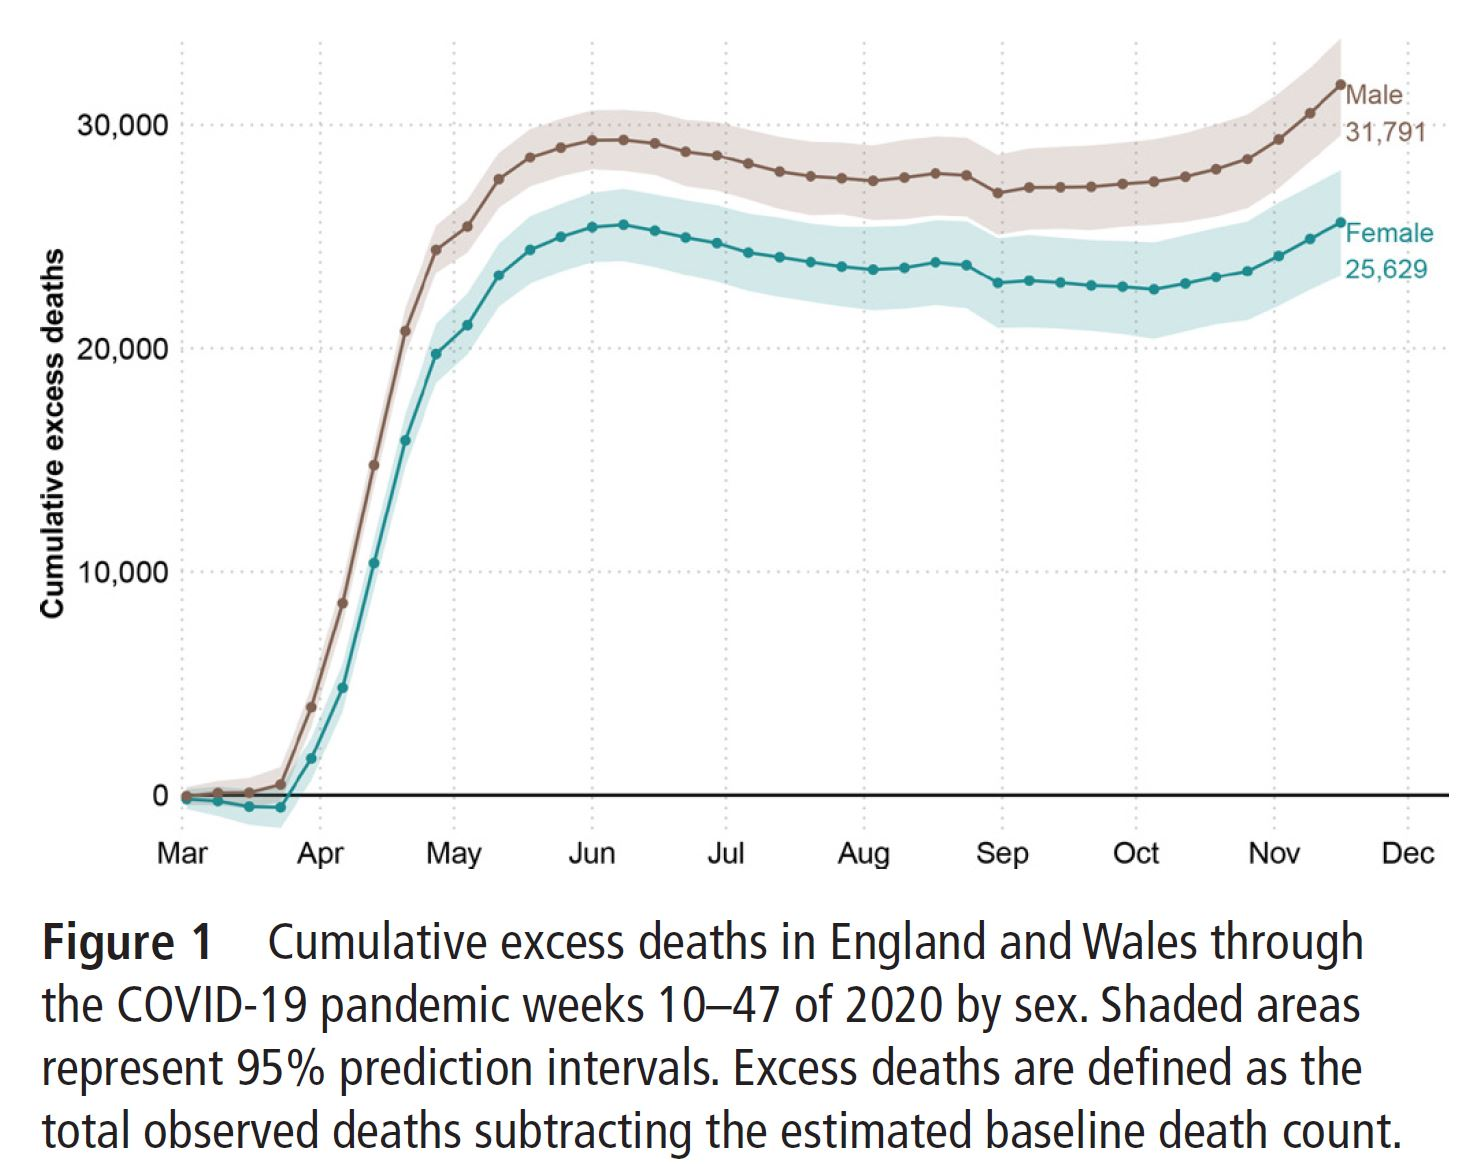
\includegraphics[width=1.2\textwidth]{Figures/Excess_England}};
		\end{tikzpicture}

	\end{column}
	
	\begin{column}{0.25\textwidth}
	
		\begin{tikzpicture}
			\node (img){
\includegraphics[width=.68\textwidth]{Figures/England_paper}};
	\end{tikzpicture}

	\end{column}
	
\end{columns}

\end{frame}



\begin{frame}
	\begin{center}
		\LARGE{\textbf{What is life expectancy?}} \pause \linebreak
	
\Large{\textcolor{darkgray}{Average number of years a \textbf{synthetic} cohort of newborns would live if they were to experience the death rates observed in a given period throughout their lifespan}} 

	\end{center}
			
\end{frame}


\begin{frame}
	\begin{center}
		\LARGE{\textbf{Why life expectancy?}} \pause \linebreak
	
	\end{center}
		\begin{itemize}
	\Large{
	\item \textcolor{blue}{Widely used metric of population health.}
	\item \textcolor{blue}{Comparable across countries and over time.}
	\item \textcolor{blue}{Summarized mortality in a given year.}
	\item \textcolor{blue}{Decomposable with demographic methods.}
	}
	\end{itemize}
	
		
\end{frame}

\begin{frame}
	\begin{center}
		\LARGE{\textbf{Objective}} \linebreak
		
\Large{\textcolor{darkgray}{To go beyond excess deaths and country-specific analyses and focus on the pressing issue of revealing the impacts of the pandemic on life expectancy in a cross-national perspective.}} \pause \linebreak

	\end{center}
	
\Large{\textcolor{red}{Initial challenge: Data, consistency, estimates of mortality by age.}}
	
		
\end{frame}



\begin{frame}

\begin{center}
 \LARGE{\textbf{Life expectancy at birth 2015-19}}
\end{center}

\begin{columns}

\begin{column}{0.65\textwidth}
\vspace*{-.8cm}
 \begin{tikzpicture}
\node (img) {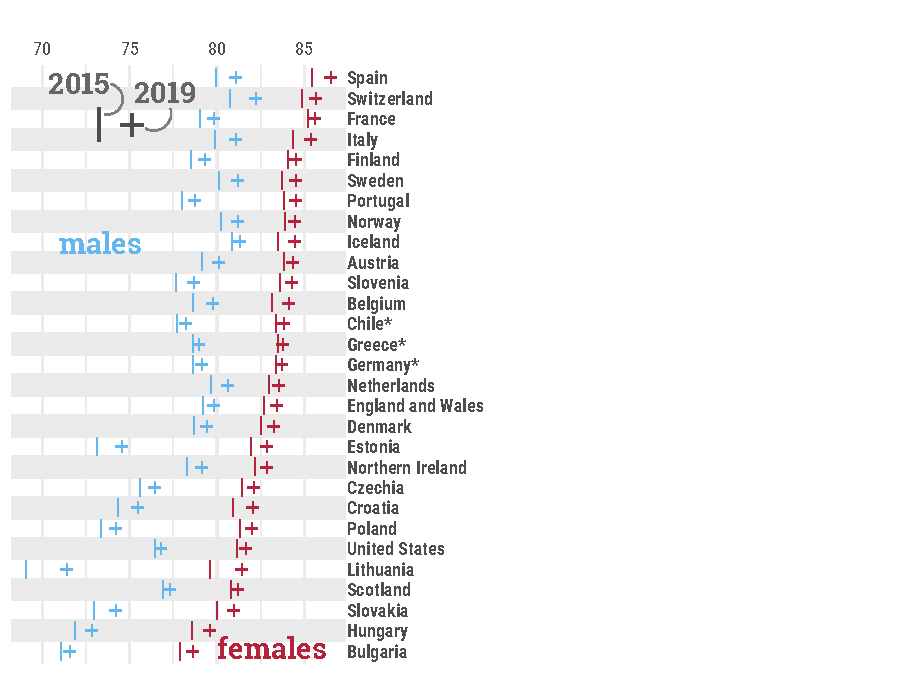
\includegraphics[width=1.65\textwidth]{Figures/fig 1_final}};
\end{tikzpicture}

\end{column}

\pause

\begin{column}{0.35\textwidth}
\vspace*{-.8cm}

\Large{

\begin{center}\textbf{Some observations}\\
\end{center}
\textcolor{darkgray}{
Females $>$ Males  \linebreak \\
Most with improvements 2015-19 \linebreak \\
Eastern Europe, Scotland, USA lagging behind 
}
}
\end{column}
\end{columns}  
\end{frame}


\begin{frame}
\begin{center}
 \LARGE{\textbf{Life expectancy losses in 2020}}
\end{center}

\begin{columns}

\begin{column}{0.65\textwidth}
\vspace*{-.5cm}
 \begin{tikzpicture}
\node (img) {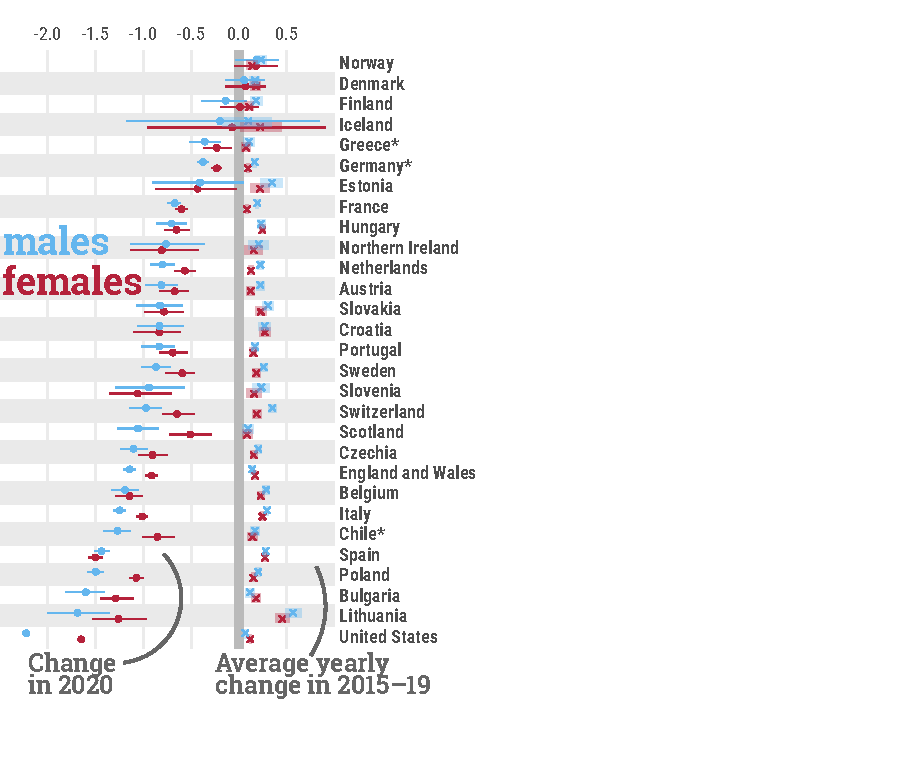
\includegraphics[width=1.5\textwidth]{Figures/fig 2_final}};
\end{tikzpicture}

\end{column}

 \pause

\begin{column}{0.35\textwidth}
\vspace*{-.8cm}

\Large{

\begin{center}\textbf{Some observations}\\
\end{center}

\textcolor{darkgray}{
12 countries with over 1 year of loss \linebreak \\
males $>$ females \linebreak \\
Scandinavia (-SWE) success cases
}}
\end{column}
\end{columns}  
\end{frame}



\begin{frame}
\begin{center}

 \LARGE{\textbf{How big? In historical context}}
 
 	\animategraphics[height=2.2in,controls = play]{12}{imgpdf/animate_}{0}{299}
												

\end{center}
\end{frame}


\begin{frame}

\begin{center}
 \LARGE{\textbf{Age specific-contributions}}
\end{center}

\begin{columns}

\begin{column}{0.5\textwidth}
\begin{center}
\vspace*{-.8cm}
\LARGE{Females}\\
\begin{tikzpicture}
\node (img) {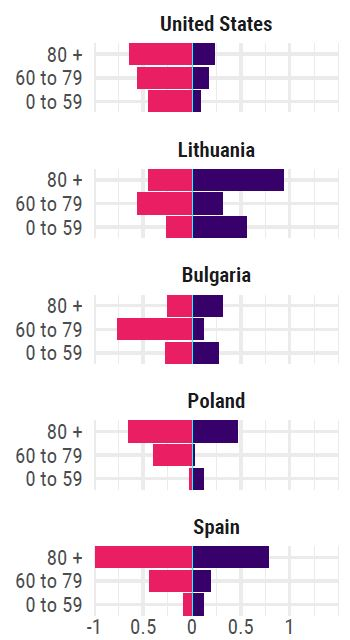
\includegraphics[width=.60\textwidth]{Figures/Decomp_1}};
\end{tikzpicture}
\end{center}
\end{column}

\pause

\begin{column}{0.5\textwidth}
\begin{center}
\vspace*{-.8cm}
\LARGE{Males}\\
 \begin{tikzpicture}
\node (img) {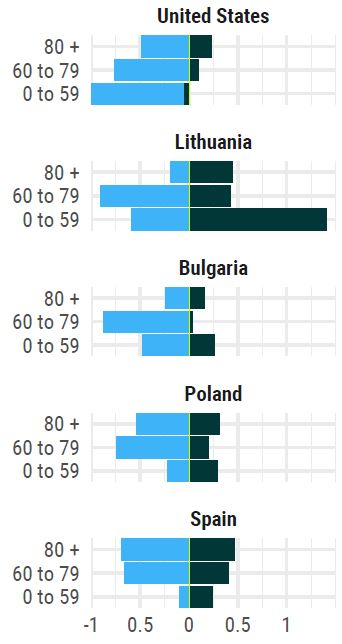
\includegraphics[width=.59\textwidth]{Figures/Decomp_2}};
\end{tikzpicture}
\end{center}
\end{column}

\end{columns}  
\end{frame}

\begin{frame}
\begin{center}
 \LARGE{\textbf{COVID-19 contribution}}
\end{center}


 \begin{tikzpicture}
\node (img) {\hspace*{0.5cm}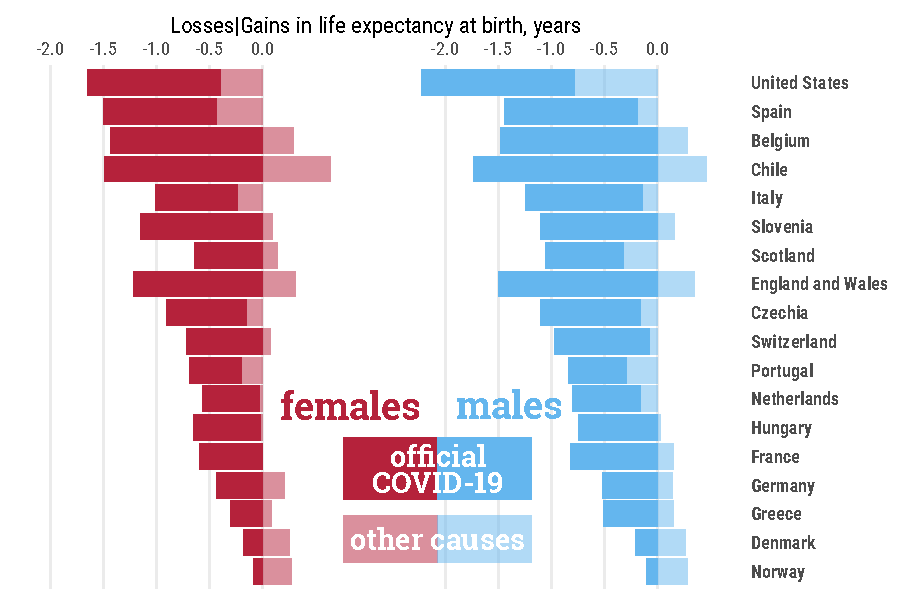
\includegraphics[width=1\textwidth]{Figures/fig 5_final}};
\end{tikzpicture}

\end{frame}







%%%%%%%%%%%%%%%%%%%%%%%%%%%%%%%%%%%%%%%%%%%%%%%%%%%%%%%%%%%%%%%%%%%%%%%%

%%%%%%%%%%%%%%%%%%%%%%%%%%%%%%%%%%%%%%%%%%%%%%%%%%%%%%%%%%%%%%%%%%%%%%%%
\begin{frame}
 \begin{center}

			\color{black}\Large{\textbf{Jos\'{e} Manuel Aburto}}\\	
				
		\faEnvelope: jose-manuel.aburto@sociology.ox.ac.uk\\		
			\faTwitter \quad @jm\_aburto  @OxfordDemSci and @CPop\_SDU \\
			\faGithub \quad @jmaburto 
			$\,$\\
						$\,$\\
						 	\animategraphics[height=2.2in,controls = none,autoplay]{12}{imgpdf/animate_}{0}{299}
						\end{center}
						
					





 
 

\end{frame}

\end{document}
	

